\documentclass[../main.tex]{subfiles}

\begin{document}

\subfile{sections/submethods/method_introduction}


\subsection{Preprocessing and parallelism}
Compute priors for $m$ and store somewhere where all processes can read. (shared memory, file)\\[1em]
Create unique identifiers for each cell. Each cell should be in own aligned BAM file.\\[1em]
Pile up aligned BAMs on loci.
\begin{itemize}
    \item Use Python's PySam pileup to iterate through columns (loci).
    \item Workers pick up batches of 1000? loci. Since sites assumed to be independent (note: should they be?) synchronicity is not important if locus positions and cellIDs are tracked.
    \item Workers process batch through to genotype calculation so not all are on I/O at once.
    \item Return locus objects with cells' read and qual info at that locus.
\end{itemize}
\vspace{1em}
Mark or discard indels and low/no coverage.\\[1em]
Impute welltype from germline data.
\begin{itemize}
    \item If germline VCF file provided, impute here
    \item If no germline VCF, if cell consensus (likelihood threshold?) different than reference, impute
    \item Optionally use dbSNP as prior for germline vs somatic mutation
\end{itemize}
\subsection{Cell genotype likelihoods}
Calculate genotype likelihoods for each cell $j$ at each locus $i$. We assume independence between sites.
\subsubsection*{Homozygous genotypes}
\begin{itemize}
    \item Let $g\in\{0,1,2\}$ be the unphased genotype of a locus designated by the number of non-reference alleles. For homozygous genotypes (that is, $g\in\{0,2\}$) We generally assume reads to be independent:
    \begin{equation}
        P(D_{ij}\mid g) = \prod_{k=1}^n P(d_{ijk} \mid g)
    \end{equation}
    Note $D_{ij}=(\vec{r},\vec{e})$, where $\vec{r}$ are the $n$ reads at this nucleotide and this cell. $\vec{e}$ are the associated probabilities of read error, derived from the phred quality scores.\\
    \item Marginalizing on sequencing error:
    \begin{equation*}
        P(d_k \mid g) =  P(r_k,\,se \mid g) + P(r_k,\,\neg se \mid g)
    \end{equation*}
    \item Since errors can occur during amplification or sequencing, we model an "intermediate allele", denoted $\beta$ that is amplified from the original nucleotide with some probability of error~\cite{monovar}. Trivially:
    \begin{equation*}
        P(r_k,\,\neg se \mid g) = P(r_k\mid \neg se ,\, g)(1-e_k)=P(\beta_k=r_k\mid g)(1-e_k) 
    \end{equation*}
    We similarly see:
    \begin{equation*}
        P(r_k,\, se \mid g) = P(r_k\mid se,\, g)e_k
    \end{equation*}
    Furthermore:
    \begin{equation*}
        P(r_k\mid se,\, g) = P(r_k\mid \beta_k\neq r_k,\,se,\,g) P(\beta_k\neq r_k \mid se,\,g)
    \end{equation*}
     Assuming (?) an error in sequencing the intermediate allele could produce any of the other three alleles with equal probability we find $P(r_k\mid \beta_k \neq r_k,\,se,g)=1/3$. Since the amplification of $\beta$ is unaffected by sequencing $P(\beta_k\neq r_k \mid se,\,g)=P(\beta_k\neq r_k\mid g)=1-P(\beta_k=r_k\mid g)$. We therefore have:
     \begin{equation*}
         P(r_k, se \mid g) = e_k \frac{1}{3}\left[1-P(\beta_k=r_k\mid g)\right]
     \end{equation*}
     \item Finally the likelihood $P(D_{ij}\mid g)$ for cell at a locus for a homozygous genotype is:
     \begin{equation}
          P(D_{ij}\mid g) = \prod_{k=1}^n \left[ (1-e_k)P(\beta_k=r_k\mid g) + e_k \frac{1}{3} (1-P(\beta_k=r_k\mid g)) \right]
     \end{equation}
\end{itemize}
\subsubsection*{Heterozygous genotypes and allelic dropout}
\begin{itemize}
     \item For the heterozygous case, we must account for the possibility of allelic dropout (ADO)~\cite{monovar,sciphi}. Therefore:
     \begin{equation*}
         P(D_{ij}\mid g=1) = P(D_{ij}, \text{ADO} \mid g=1)+ P(D_{ij}, \neg \text{ADO}\mid g=1)
     \end{equation*}
     Letting $P_{ADO}$ be the probability of an a dropout event, this expands to:
     \begin{equation*}
         P(D_{ij}\mid g=1) = P_{ADO}P(D_{ij}\mid \text{ADO},\, g=1) + (1-P_{ADO})P(D_{ij} \mid \neg \text{ADO},\, g=1)
     \end{equation*}
     In the result of an allelic dropout from a heterozygous locus, only one allele will remain after the amplification process and hence the likelihood $P(D_{ij}\mid \text{ADO},\, g=1)$ will resemble the homozygous case. We assume allelic dropout can affect either  allele with equal probability and hence:
     \begin{equation*}
         P(D_{ij}\mid \text{ADO},\, g=1) =\frac{1}{2}P(D_{ij}\mid g=0) + \frac{1}{2}P(D_{ij}\mid g=2)
     \end{equation*}
     For the case without allelic dropout, the form of the likelihood is identical to the homozygous case:
     \begin{equation*}
           P(D_{ij}\mid \neg\text{ADO},\,g=1) = \prod_{k=1}^n \left[ (1-e_k)P(\beta_k=r_k\mid g=1) + e_k \frac{1}{3} (1-P(\beta_k=r_k\mid g=1)) \right]
     \end{equation*}
\end{itemize}
%NOTE: for thesis good to include all calculation but for paper should probably just cite monovar

\subsection{Mutated site priors}
We now focus on the prior probability of the total alternate allele count being $\sigma$ at the locus under consideration: $P(\sum_j g_{ij}=\sigma)=P(\sigma)$. The majority of sites will not include a somatic SNV (sSNV); we say that any site has a prior probability $\lambda$ of having a somatic SNV, which is set to 0.0001 by default~\cite{monovar, sciphi}. %This is for SNPs, accurate for SNVs? Does it matter? SciPHI says no. Perhaps tune hyperparameter from real data.
%
%NB truncal comes from metastatic prostate Gundem et al. NOT strictly true i.e. clonal SNV or SNP(!) with LOH in tree? %TODO : include case of truncal SNV but somatic LOH!
\begin{equation} \label{eq:overallprior}
P(\sigma)=P(\sigma\mid\text{sSNV})\lambda+P(\sigma\mid\neg\text{sSNV})(1-\lambda)
\end{equation}
Any given sample of single cells will only represent some subtree of a full cell phylogeny. As such, when considering the case where there is a sSNV at the locus we can further break down the prior into the case where the sSNV is ancestral to all sampled cells and the case where where the SNV occurs within the subtree rooted at the most recent common ancestor (MRCA) of the cells sampled. We denote the case where the mutation occurs within this subtree as $\text{SNV}_T$.
\begin{equation} \label{eq:somaticsnv}
P(\sigma\mid\text{sSNV})=P(\sigma\mid \text{SNV}_T)P(\text{SNV}_T\mid \text{sSNV})+P(\sigma\mid \text{sSNV},\,\neg\text{SNV}_T)(1-P(\text{SNV}_T\mid \text{sSNV}))
\end{equation}
\subsubsection*{Ploidy changes}
It is well known that many tumor cells may exhibit aneuploidy or chromosomal abnormaities~\cite{gao2016punctuated,21breasts}. For simplicity, we will disregard polyploidy and focus only on the case where loci become haploid. This sort of mutation can result in lost information regarding SNVs, as a loss of heterozygosity can lead to a locus being read as homozygous~\cite{sciphi}. Note that this is an in vivo effect, distinct from allelic dropout which occurs in vitro during DNA ampification. We will model such occurences as a sudden switch to homozygosity, as we cannot reliably distinguish diplod homozygosity from haploidy in the genomic SCS data, which already has significantly uneven coverage and depth~\cite{scprimer}. Let $H$ be the event that the locus under examination has become haploid, and $H_T$ be the case that this mutation has occured within subtree rooted at the MRCA of all sequenced cells.
\begin{equation}
P(\sigma \mid \text{SNV}_T) = P(\sigma\mid\text{SNV}_T,H)P(H) + P(\sigma\mid\text{SNV}_T,\neg H)(1-P(H)) 
\end{equation}
%TODO no prior on P(H). Set as same as lambda? No, in most cancers seems like almost half have CNAs (Gao et al). Also todo remove "initially" from next sentence if don't reestimate
We initially set the value of $P(H)$ to .09 (See Appendix A). In the simplest case, we consider the prior probability of an alternate allele count of $\sigma$ given a mutation occured within the subtree and the locus remained diploid across all sampled cells. Assuming infinite sites, in such a scenario mutations would only be heterozygous.
\begin{equation*}
P(\sigma\mid\text{SNV}_T,\neg H) = \begin{cases} \frac{2m-1}{2(m-1)} T(m,\sigma) \qquad 0<\sigma< m\\ 0 \qquad \qquad \quad \text{else}\end{cases}
\end{equation*}
Where $T(m,\sigma)$ is the prior developed by Singer, Kuipers et al. that assumes a mutation may occur on any branch of the sampled subtree with equal probability.
\begin{equation}
T(a,b)=\frac{\binom{a}{b}^2}{(2b-1)\binom{2a}{2b}}
\end{equation}
Now let us consider the case where both a sSNV and a haploid event have both occured at a locus. Since the haploid mutation may have occured in the subtree or ancestral to the subtree, we model these cases seperately.
\begin{equation*}
P(\sigma\mid\text{SNV}_T,H) = P(\sigma\mid\text{SNV}_T,H_T)P(H_T\mid H) + P(\sigma\mid\text{SNV}_T,H,\neg H_T)(1-P(H_T\mid H)) \label{eq:SNVT}
\end{equation*}
\subsubsection*{SNV and loss of heterozygosity within the subtree}
In the first scenario described by Equation~\ref{eq:SNVT} both a point mutation and a ploidy change have occured within the sequenced subtree. This can be split into four further subcases (Figure~\ref{fig:bothmutationstree}).

\begin{figure}[h]
	\centering

	\begin{subfigure}{0.2\textwidth}
		\centering
		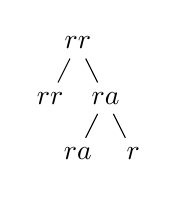
\begin{tikzpicture}[sibling distance=2em, level distance=2em]
  \node {$rr$}
    child { node {$rr$} }
    child { node {$ra$}
      child { node {$ra$} }
      child { node {$r$}}
          };
		\end{tikzpicture}
		\caption{Case 1}
	\end{subfigure}
	\begin{subfigure}{0.2\textwidth}
		\centering
		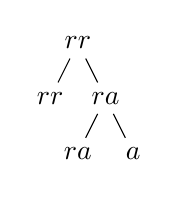
\begin{tikzpicture}[sibling distance=2em, level distance=2em]
  \node {$rr$}
    child { node {$rr$} }
    child { node {$ra$}
      child { node {$ra$} }
      child { node {$a$}}
          };
		\end{tikzpicture}
		\caption{Case 2}
	\end{subfigure}
	\begin{subfigure}{0.2\textwidth}
		\centering
		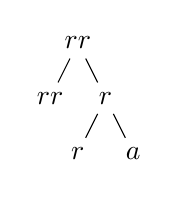
\begin{tikzpicture}[sibling distance=2em, level distance=2em]
  \node {$rr$}
    child { node {$rr$} }
    child { node {$r$}
      child { node {$r$} }
      child { node {$a$}}
          };
		\end{tikzpicture}
		\caption{Case 3}
	\end{subfigure}
	\begin{subfigure}{0.2\textwidth}
		\centering
		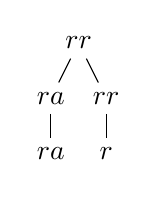
\begin{tikzpicture}[sibling distance=2em, level distance=2em]
  \node {$rr$}
    child { node {$ra$} 
    	child { node {$ra$} }
    	  }
    child { node {$rr$} 
    	child { node {$r$} }
    	};
		\end{tikzpicture}
		\caption{Case 4}
	\end{subfigure}
	
	\caption{SNV and haploid event both within the subtree. (a) Point mutation happens before haploid event and mutated allele is dropped. (b) Point mutation happens before haploid event and reference allele is dropped. (c) Haploid event occurs before point mutation. Since haploid cells are modelled as becoming homozygous diploids, this case leads to only even values of alternate allele count. (d) In this case the point mutation and haploid event do not occur in the same lineage. We ignore this case as the haploid event does not affect the alternate allele count.}
\label{fig:bothmutationstree}
\end{figure}
Considering the above three cases where a ploidy change in the subtree affects the locus alternate allele count, it is twice as likely that the point mutation should occur before the haploid event (cases 1 and 2), compared with the other temporal ordring (case 3). Therefore $P(\text{case 1 or 2})=2/3$ and $P(\text{case 3})=1/3$. This is because the cells before a haploid event, being diploid, have twice the chance of having a point mutation at a locus than the haploid descendants of such a mutation. We also assume the refence and alternate alleles have an equal chance of being dropped in a loss of heterozygosity.
\begin{equation*}
P(\text{case 1})=P(\text{case 2}) = P(\text{case 3}) = 1/3
\end{equation*}
Continuing to assume that both a point mutation and a haploid event have occured within the sequenced subtree at the locus in question, we now have
\begin{equation*}
P(\sigma\mid\text{SNV}_T,H_T)=\frac{1}{3}\left[P(\sigma\mid\text{case 1})+P(\sigma\mid\text{case 2})+P(\sigma\mid\text{case 3})\right]
\end{equation*}
To examine these probabilities we will use the function $T(a,b)$ described above, which given a subtree with $a$ leaves gives the probability of a mutation affecting $b$ of those leaves. For case 1, the loss of heterozygosity effectively deletes all alternate alleles from the cells sharing a lineage with the haploid event, and so
\begin{equation*}
P(\sigma\mid\text{case 1}) = \frac{1-2m}{2(1-m)}\sum_{a-h=\sigma}T(m,a)T(a,h)\qquad 1\leq a < m,\;1\leq h\leq a
\end{equation*}
%TODO : Very slow computation!!
While we include one normalization constant, excluding the case of an ancestral point mutation, we do allow the case where a point mutation and a loss of heterozygosity happen on the same branch of the phylogeny. Hence the support for $\sigma$ in case 1 is $[0,m)$. Since we model a haploid event as a sudden switch to homozygosity, the observed allele count for case 2 is the number of cells affected by the heterozygous point mutation ($a$) added to the number of cells affected by the loss of heterozygosity ($h$).
\begin{equation*}
P(\sigma\mid\text{case 2}) = \frac{1-2m}{2(1-m)}\sum_{a+h=\sigma}T(m,a)T(a,h) \qquad 1\leq a < m,\;1\leq h\leq a
\end{equation*}
For case 2, the support is [2,\,2m-2]. In case 3, only even allele counts can be produced as all cells carrying the point mutation are haploid, which we model as being homozygous mutated. The possible values of $\sigma$ are $1\leq\sigma\leq 2m-2$.
\begin{equation*}
P(\sigma\mid\text{case 3}) = \frac{1-2m}{2(1-m)}\sum_{2a=\sigma} T(m,h)T(h,a) \qquad 1\leq h < m,\; h\geq a
\end{equation*}
\subsubsection*{Haploid subtree}
Referreing back to Equation~\eqref{eq:SNVT}, we must determine the prior probability of an alternate allele count $\sigma$ at a locus given that a point mutation occured within the sequenced subtree and a haploid event occured ancestral to the subtree. This would lead to all sampled cells being haploid at this locus, therefore allowing only even allele counts.
\begin{equation*}
P(\sigma\mid \text{SNV}_T,H,\neg H_T) = \begin{cases} \frac{2m-1}{2(m-1)}T(m,\frac{\sigma}{2})\qquad 2\mid\sigma,\;0<\sigma<2m\\ 0 \qquad\qquad\qquad\quad \text{else} \end{cases}
\end{equation*}
\subsubsection*{Clonal and subclonal mutations}
We have so far considered the case where sSNVs have been subclonal: they may affect some of our sampled cells and not others. There is some probability however that a sSNV at a given locus may be due to a mutation in a cell ancestral to all sampled cells. The majority of these ancestral mutations will affect all tumour cells: so-called clonal, truncal or public mutations~\cite{neutralevoltumour, 21breasts, metastatic}. If the sample of single cells is small enough, however, it could be the case that a subclonal mutation is common to all cells sampled.
\begin{equation}
P(\text{ancestral}\mid \text{sSNV})=P(\text{clonal})+P(\text{ancestral}\mid \text{subclonal})(1-P(\text{clonal}))
\end{equation}
To find the probability of a subclonal mutation affecting all sampled cells, we assume tumour subclones follow a neutral evolutionary model such that subclonal mutant allele frequencies follow a power law distribution~\cite{neutralevoltumour}. Using an IID model for tumour cell sampling, the probability that all $m$ cells are from a subclone with cellular frequency $2f$ (allelic frequency = $f$) is $(2f)^m$. Similar to Williams et al. we define a probability density function for the allelic frequency of subclonal mutations proportional to the inverse of the allelic frequency.\\
%TODO how can assume heterozygosity??)
\begin{equation}
P(f) = k\left(\frac{1}{f}-2\right)
\end{equation}
where $k$ is a normalization constant. We define the support of $P(f)$ for subclones as $[10^{-8},0.5]$, as a frequency of $10^{-8}$ is on the order of affecting single cells and an allelic frequency of $0.5$ corresponds to clonal mutations~\cite{numcells}. We find a value of $k$ by integrating $P(f)$ over this support. If a subclonal mutation affects all sampled cells, then all these cells must be from the same subclone.
\begin{equation} \label{eq:tmids}
P(\text{ancestral}\mid \text{subclonal}) = \int_f P(\text{all in subclone}\mid f)P(f)\,df=\int_{10^{-8}}^{0.5}(2f)^mk\left(\frac{1}{f}-2\right)\,df
\end{equation}
For large enough samples ($m>30$) the probability that all cells were sampled from a single subclone (Equation~\ref{eq:tmids}) becomes negligible. Since it is only a function of $m$ these values are pre-computed for efficiency. The empirically estimated probability that any given mutation is clonal is set at $P(\text{clonal})=0.51$ (see appendix A)~\cite{21breasts, metastatic, yachida}. Having developed the probability that any given somatic mutation is ancestral to all sampled cells, we have also found the probability that a mutation has occured within the sampled subtree.
\begin{equation*}
P(\text{SNV}_T\mid\text{sSNV})=P(H_T\mid H)=1-P(\text{ancestral}\mid\text{sSNV})
\end{equation*}

\subsubsection*{Ancestral sSNVs}
Referring Equation~\eqref{eq:somaticsnv} we must also determine the prior for $\sigma$ in the case that the sSNV is ancestral to all cells. Without LOH this would always result in $\sigma=m$, however we must again consider haploid events both within and ancestral to the sampled subtree.
\begin{equation} \label{eq:ancestralsnv}
P(\sigma\mid\text{sSNV},\,\neg\text{SNV}_T)=P(\sigma\mid\text{sSNV},\,\neg\text{SNV}_T,\,H)P(H)+P(\sigma\mid\text{sSNV},\,\neg\text{SNV}_T,\,\neg H)(1-P(H))
\end{equation}
If there is no haploid event, there will be no LOH and the ancestral sSNV will be heterozygous across all cells.
\begin{equation*}
P(\sigma\mid\text{sSNV},\,\neg\text{SNV}_T,\,\neg H) = \begin{cases}1\quad \sigma=m\\ 0\quad\text{else}\end{cases}
\end{equation*}
In the case of a haploid event, we must consider the cases where the whole subtree is haploid and when the haploid event happens within the subtree. We also consider the alternate and reference alleles to be dropped with equal probability as above.
\begin{equation*}
P(\sigma\mid\text{sSNV},\,\neg\text{SNV}_T,\,H)=(1-P(H_T\mid H))P(\sigma\mid H,\,\neg H_T)+P(H_T\mid H)P(\sigma\mid H_T,\,\text{SNV},\,\neg\text{SNV}_T)
\end{equation*}
If both the somatic SNV and the haploid event are ancestral to the sequenced subtree, the cells will either all be haploid reference or all be haploid alternate with equal probability. Since we model haploid cells as homozygous diploid this results in only alternate allele counts of $0$ or $2m$.
\begin{equation*}
P(\sigma\mid\text{SNV},\,\neg\text{SNV}_T,\,H,\,\neg H_T)= \begin{cases} \frac{1}{2} \quad \sigma=0,2m\\0\quad \text{else} \end{cases}
\end{equation*}
If there is an sSNV ancestral to the sampled cells but a haploid event occured within the sampled subtree we may have any alternate allele count from $1$ to $2m-1$ depending on where in the phylogeny heterozygosity was lost and which allele was dropped.
\begin{equation*}
P(\sigma\mid\text{SNV},\,\neg\text{SNV}_T,\,H_T) = \begin{cases} \frac{1}{2}T(m,\sigma-m)\qquad \sigma > m\\
\frac{1}{2}T(m,m-\sigma)\qquad m > \sigma \end{cases}
\end{equation*}

\subsection{Welltype site priors}
We have so far considered the prior probability of alternate allele counts at a locus given that a somatic SNV has occured at that locus. The majority of loci, however, will be unaffected by sSNVs, although may still contain germline point mutations. Referring back to Equation~\eqref{eq:overallprior} we must consider the prior probabilities of $\sigma$ for sites without sSNVs. Note, however, that such a site may still be affected by anneuploidy.
\begin{equation}
P(\sigma\mid\neg\text{sSNV})=P(\sigma\mid\neg\text{sSNV},H)P(H)+P(\sigma\mid\neg\text{sSNV},\neg H)(1-P(H))
\end{equation} 
In the case where there is no sSNV and no anneuploidy, we simply assume Hardy-Weinberg equilibrium, with a germline mutation rate of $\mu$. We set the value of $\mu$ relatively high at $0.1$ to reduce false positive errors.
%TODO this is something to test. Grid search all parameter space on new data.\\
\begin{equation*}
P(\sigma\mid\neg\text{sSNV},\,\neg H) = \begin{cases} \mu^2\qquad\qquad\quad\,\sigma=2m\\ 2\mu(1-\mu) \qquad \sigma = m \\ (1-\mu)^2 \qquad \; \;\, \sigma=0 \\ 0 \qquad\qquad\quad\;\;\; \text{else} \end{cases}
\end{equation*}
Continuing to assume HWE for the germline genotype, anneuploidy will only affect the alternate allele count for a heterozygous germline genotype. Here again we assume either allele may be dropped with equal probability.
\begin{equation*}
P(\sigma\mid\neg\text{sSNV},\, H) = \begin{cases} \mu^2 + \mu(1-\mu)(1-P(H_T\mid H))\qquad\qquad\quad\;\; \sigma=2m\\
\mu(1-\mu)P(H_T\mid H)\frac{2m-1}{2(m-1)}T(m,m-\sigma) \qquad 0<\sigma<m\\
0 \qquad\qquad\qquad\qquad\qquad\qquad\qquad\qquad\qquad\quad \sigma=m \\
\mu(1-\mu)P(H_T\mid H)\frac{2m-1}{2(m-1)}T(m,\sigma-m) \qquad\;\; m<\sigma<2m\\
(1-\mu)^2 + \mu(1-\mu)(1-P(H_T\mid H)) \qquad\qquad \sigma=0 \end{cases}
\end{equation*}

\subsection{Variant site calling}
To improve algorithmic efficiency we wish only to consider sites with a non-trivial posterior probability of containing a somatic mutation. Furthermore it has been shown that combining low coverage sequencing data across samples at a locus can decrease false positive rates~\cite{ledurbin}. We therefore must reject loci where the posterior probability of mutation is low. For a given locus $i$:
\begin{equation}
P(SNV_i\mid D_i) = 1- P\left(\sum_{j=1}^m g_{ij} = 0 \mid D_i\right) = 1-P(\sigma = 0 \mid D_i)
\end{equation}
Using Bayes' formula:
\begin{equation}\label{eq:sitebayes}
P\left(\sigma = 0 \mid D_i\right) = \frac{P(D_i\mid \sigma = 0)P(\sigma = 0)}{\sum_{\sigma'=0}^{2m}[P(D_i\mid \sigma=\sigma')P(\sigma')]}
\end{equation}
The value of $P(D_i\mid \sigma = 0)$ is simply the product of the cell likelihoods of homozygous reference calculated above. The priors $P(\sigma)$ are those determined by Equation~\eqref{eq:overallprior}. To compute the denominator, howevever, we must compute the likelihood for each alternate allele count across a locus. There are various permutations of cell genotypes that may give rise to an alternate allele count of $\sigma$, so this is not as simple as the special case where $\sigma=0$.\\

Let the phased genotypes of all $m$ cells at a site be represented by $\vec{G} = (G_1,G_2,\dots,G_m)$ where $G_j\in [0,1]\times[0,1]$ is the phased genotype for cell $j$ (0 = reference, 1 = alternate). Furthermore let the unphased genotype vector be $\vec{g} = (g_1,g_2,\dots,g_m)$ be such that $g_j = \norm{G_j}_1$. Our likelihood for $\sigma$ can therefore be considered
\begin{equation} \label{eq:phasedlike}
P(D_i\mid\sigma_i) = \sum_{\vec{G}} P(D_i \mid \vec{G}) P(\vec{G} \mid \sigma_i)
\end{equation}
We assume that all phased genotype vectors with a total alternate allele count of $\sigma$ are equally probable. Since there are $\binom{2m}{\sigma}$ different phased genotype vectors with total alternate allele count $\sigma$, then for any such $\vec{G}$:
\begin{equation*}
P(\vec{G}\mid \sigma) = \binom{2m}{\sigma}^{-1}
\end{equation*}
Since we do not consider phased sequencing data, we must reproduce Equation~\eqref{eq:phasedlike} in an unphased form. To begin, we see that the likelihood $P(D_i\mid \vec{G}) = P(D_i\mid \vec{g})$ if $\vec{g}$ is the unphased vector that corresponds to $\vec{G}$, since our cell genotype likelihoods do not consider phasing. Note that there are $2^\chi$ phased genotype vectors that correspond to any given unphased genotype vector $\vec{g}$, where $\chi(\vec{g})$ is the number of heterozygous cells in the vector. Using this multiplicity, we can now reproduce Equation~\eqref{eq:phasedlike} without reference to phasing.
\begin{equation*}
P(D_i\mid\sigma_i) = \sum_{\vec{g}} \frac{2^{\chi(\vec{g})}}{\binom{2m}{\sigma_i}} P(D_i\mid\vec{g}) = \sum_{\vec{g}} \frac{2^{\chi(\vec{g})}}{\binom{2m}{\sigma_i}} \prod_{j=1}^{m}P(D_{ij}\mid g_{j})
\end{equation*}
Let the function $\delta(\vec{g},\sigma) = 1$ if $\norm{\vec{g}}=\sigma$ otherwise it evaluates to 0. We can now write the above in a more suggestive form:
\begin{equation}\label{eq:sitelikelihood}
P(D_i\mid\sigma_i) = \binom{2m}{\sigma_i}^{-1}\sum_{g_1=0}^2\sum_{g_2=0}^2\dots\sum_{g_m=0}^2 \delta((g_1,\dots g_m),\sigma_i)\left[\prod_{j=1}^{m}\binom{2}{g_j}P(D_{ij}\mid g_{j})\right]
\end{equation}
As has been done previously, we can employ a dynamic programming approach to compute these likelihoods for $\sigma$ from cell genotype likelihoods~\cite{monovar, sciphi, ledurbin}. If we let $F(k,l)$ be the subproblem objective given by
\begin{equation}
F(k,l) = \begin{cases} \sum_{g_1=0}^2\sum_{g_2=0}^2\dots\sum_{g_k=0}^2 \delta((g_1,\dots g_k),l)\left[\prod_{j=1}^{k}\binom{2}{g_j}P(D_{ij}\mid g_{j})\right] \quad 0\leq l \leq 2k \\
0 \qquad\qquad\qquad\qquad\qquad\qquad\qquad\qquad\qquad\qquad\qquad\qquad\qquad\qquad \text{else} \end{cases}
\end{equation}
We can consider creating a genotype vector of length $k$ from a vector of length $k-1$ by adding one new cell with an alternate allele count of $0,1$ or $2$. Hence our recurrence relation can be given by
\begin{equation}
F(k,l) = F(k-1,l)P(D_{ik}\mid g_k = 0) + 2F(k-1,l-1)P(D_{ik}\mid g_k = 1) + F(k-1,l-2)P(D_{ik}\mid g_k = 2)
\end{equation}
Note that two possible phased genotypes correspond to the heterozygous case, hence the factor of 2 in the second term. The base case where $k=1$ corresponds to a single cell
\begin{equation*}
F(1,0) = P(D_{i1}\mid g_1 = 0),\;\; F(1,1) = 2P(D_{i1}\mid g_1=1),\;\; F(1,2) = P(D_{i1}\mid g_1 = 2)
\end{equation*}
The values for $F(k,l)$ are memoized in an array and the likelihood given in Equation~\ref{eq:sitelikelihood} can be given by
\begin{equation}
P(D_i\mid \sigma_i)=\frac{F(m,\sigma_i)}{\binom{2m}{\sigma_i}}
\end{equation}
In this way we can determine the likelihood of all $0\leq \sigma\leq 2m$ which when the priors $P(\sigma)$ compose the sum in Equation~\eqref{eq:sitebayes}.

Sites which have a posterior probability of being variant greater than 0.5(???) will be called as variant.
%TODO important parameter! how many to call?? will have to test this... Call fewer and faster tree joining, call more and more data to work with... also possibly more noise.
%\subsection{Summarisation of ignored loci}
%don't know if this is needed, apart from perhaps a simple count. These will all be considered homo ref, right?
\subsection{Building a cell phylogeny}
The most accurate phylogenetic structure of the sampled tumour cells could be found by searching through the entire tree space and finding a tree that maximizes likelihood or posterior probability. If $s$ mutant sites are called in the previous step there are $(2m-3)!!(2m-1)^s$ trees in the search space making this approach infeasible, leading a previous phylogeny aware approach to adopt a more efficient Markov chain Monte Carlo (MCMC) algorithm. Even this more efficient approach, however, can be quite slow, with an approximate runtime of $O(nm^3\log(m))$~\cite{sciphi}.

Instead, we use a simple neighbour-joining algorithm to quickly infer a cell phylogeny.\\

For now, build tree based just on cell likelihoods. Later update this to posteriors based on site posteriors. The ``proper" way can be found in monovar under ``Genotyping of sigle cells". Another way could be to sum over sigma with some simple formula like binomial (implies certain non existant independence).\\

Is there a way to use the DP values? frequency based?\\\\

%TODO workout actual runtimes to see how much this saves..
\subsection{Parameter reestimation and second cell phylogeny}
is this necessary? Overall mutation rate, $P(H_t\mid H),\,P(H),\,\lambda,\,P(SNP_T\mid SNP),\,\dots$\\
To some extent can be derived from papers like 21 breasts and metastatic. Can be reestimated?\\
do we just reestimate parameters or update priors on cell loci? updating priors could be fun, but maybe wait til completed to see if it brings additional benefit.\\

\subsection{Mutation tree inference}
Pairwise test from cell tree. Maximum parsimony inspired? Minimal way to create perfect phylogeny from cell phylogeny?
\subsection{Genotyping single cells}
Use probabilistic mutation tree as a prior, DFS
\subsection{Additional computational methods}
Stirlings approximation for $T(a,b)$. Pre computation /memoization of priors where possible. Log space.


\end{document}
